\documentclass{article}
\usepackage{graphicx}
\usepackage{tikz}
\usepackage{tikzsymbols}
\usetikzlibrary{calc,patterns,shapes.geometric}
\usepackage{float}
\usepackage{pdflscape}
\usepackage{geometry}

\def\centerarc[#1](#2)(#3:#4:#5){\draw[#1] ($(#2)+({#5*cos(#3)},{#5*sin(#3)})$) arc (#3:#4:#5);}

\pagestyle{empty}
\begin{document}
	\centering
	\begin{figure}[H]
		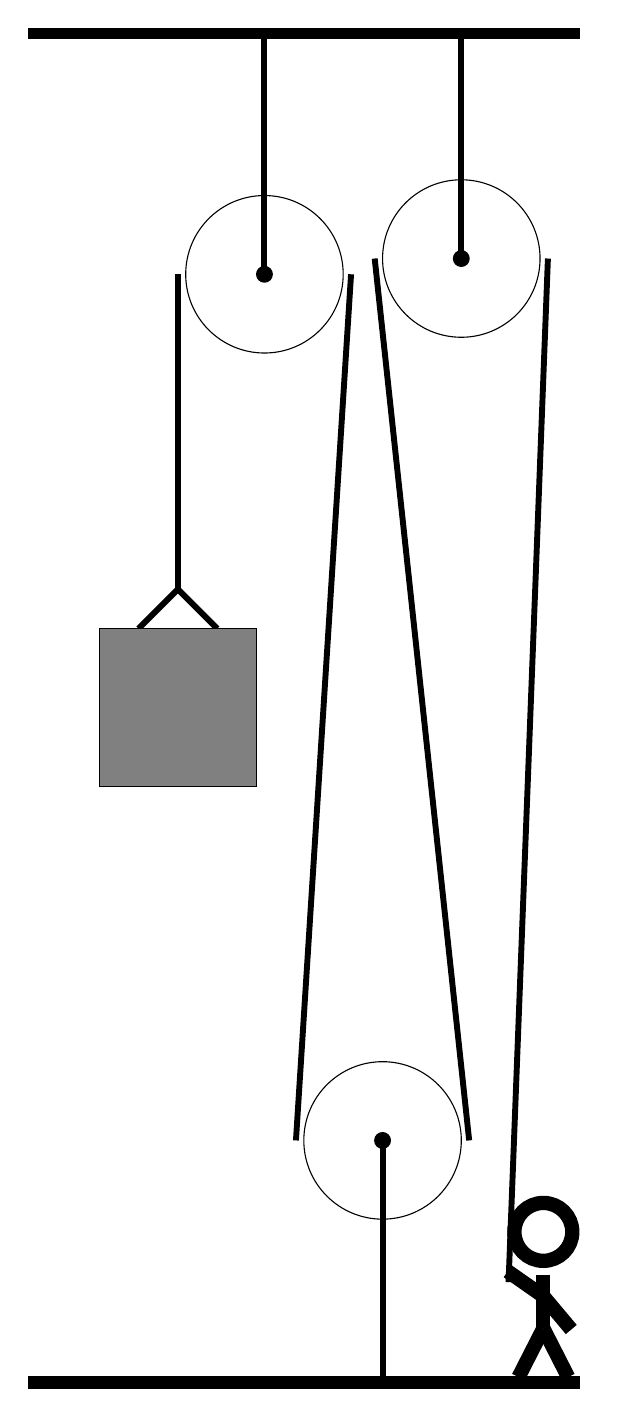
\begin{tikzpicture}
			%%%%% START %%%%%
			\def\a{14}
			\def\radlg{1}
			\def\radrp{1.1}
			\def\radsm{0.1}
			\def\yone{\a-3}
			\def\xone{1}
			\def\ytwo{\a-\a}
			\def\xtwo{2.5}
			\def\xthree{3.5}
			\def\ythree{\a*0.8}
			\def\dxtwo{9}
			\def\dx{4.5}
			\def\dy{-1.9}
			\def\dw{1.75mm}
			\def\hlena{\a*0.5}
			\def\barbump{0.2}
			\def\width{0.75mm}
			
			\draw[fill=black] (-2,\a) rectangle (5,\a+0.125); 
			
			\draw (\xone,\yone) circle (\radlg);
			\draw[fill=black] (\xone,\yone) circle (\radsm);
			\draw[line width=\width]  (\xone,\a) -- (\xone,\yone);
			
			\draw[fill=white](\xtwo,\ytwo) circle (\radlg);
			\draw[fill=black] (\xtwo,\ytwo) circle (\radsm);
			\draw[line width=\width]  (\xtwo,-3) -- (\xtwo,\ytwo);
			
			\draw[fill=white](\xthree,\ythree) circle (\radlg);
			\draw[fill=black] (\xthree,\ythree) circle (\radsm);
			\draw[line width=\width] (\xthree,\a) -- (\xthree,\ythree);
			
			\draw[line width=\width] (\xone-0.5-\radrp,\a-\hlena-0.5) -- (\xone-\radrp,\a-\hlena) -- (\xone+0.5-\radrp,\a-\hlena-0.5);
			\draw[fill=black!50] (\xone-1-\radrp,\a-\hlena-0.5) rectangle (\xone+1-\radrp,\a-\hlena-2-0.5); 
			
			\draw[line width=\width] (\xone-\radrp,\yone) -- (\xone-\radrp,\a-\hlena);
			\centerarc[line width=\width](\xone,\yone)(0:180:\radrp);
			\draw[line width=\width](\xone+\radrp,\yone) -- (\xtwo-\radrp,\ytwo);
			\centerarc[line width=\width](\xtwo,\ytwo)(180:360:\radrp);
			\draw[line width=\width](\xtwo+\radrp,\ytwo) -- (\xthree-\radrp,\ythree);
			\centerarc[line width=\width](\xthree,\ythree)(0:180:\radrp);
			\draw[line width=\width](\xthree+\radrp,\ythree) -- (\dx-0.4,\dy+0.1);
			
			\node at (\dx,\dy) {\Strichmaxerl[10][-35][-50]};
			
			\draw[fill=black] (-2,-3) rectangle (5,-3.15);
			%%%%% END %%%%%
		\end{tikzpicture}
	\end{figure}
\end{document}

